% Source PDF: source/普通高考/2015/2015全国2文(贵州,甘肃,青海,西藏,黑龙江,吉林,海南,宁夏,内蒙古,新疆,云南,广西,辽宁).pdf, page 1.
% PDF embedded-bitmap check: no image objects; the bar chart is vector content.
% Bar tops read from the source chart to the nearest 10 万吨 (no numeric labels are printed):
% 2004--2013: 2250, 2550, 2580, 2470, 2320, 2210, 2190, 2220, 2130, 2040.
% solid segments: ten bars and the rectangular frame; dashed segments: horizontal guides 2000--2600.
% Labels: years 2004--2013 and y-axis ticks 1900--2700; no answer or option text is included.

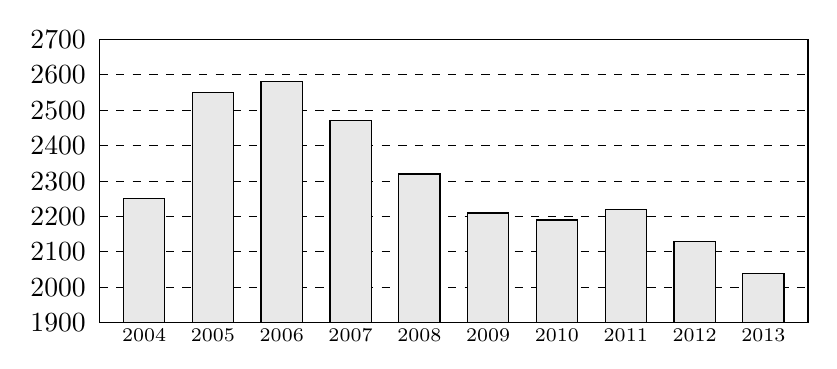
\begin{tikzpicture}
\begin{axis}[
    width=9.0cm,
    height=3.6cm,
    xmin=0.35,
    xmax=10.65,
    ymin=1900,
    ymax=2700,
    axis lines=none,
    xtick=\empty,
    ytick=\empty,
    clip=false,
    enlargelimits=false,
    scale only axis,
]
    % Horizontal guides at the labelled hundreds.
    \draw[dashed,line width=0.35pt] (axis cs:0.35,2000) -- (axis cs:10.65,2000);
    \draw[dashed,line width=0.35pt] (axis cs:0.35,2100) -- (axis cs:10.65,2100);
    \draw[dashed,line width=0.35pt] (axis cs:0.35,2200) -- (axis cs:10.65,2200);
    \draw[dashed,line width=0.35pt] (axis cs:0.35,2300) -- (axis cs:10.65,2300);
    \draw[dashed,line width=0.35pt] (axis cs:0.35,2400) -- (axis cs:10.65,2400);
    \draw[dashed,line width=0.35pt] (axis cs:0.35,2500) -- (axis cs:10.65,2500);
    \draw[dashed,line width=0.35pt] (axis cs:0.35,2600) -- (axis cs:10.65,2600);

    % Bars centred at the ten years, with heights read from the source chart.
    \draw[draw=black,fill=gray!18,line width=0.45pt] (axis cs:0.70,1900) rectangle (axis cs:1.30,2250);
    \draw[draw=black,fill=gray!18,line width=0.45pt] (axis cs:1.70,1900) rectangle (axis cs:2.30,2550);
    \draw[draw=black,fill=gray!18,line width=0.45pt] (axis cs:2.70,1900) rectangle (axis cs:3.30,2580);
    \draw[draw=black,fill=gray!18,line width=0.45pt] (axis cs:3.70,1900) rectangle (axis cs:4.30,2470);
    \draw[draw=black,fill=gray!18,line width=0.45pt] (axis cs:4.70,1900) rectangle (axis cs:5.30,2320);
    \draw[draw=black,fill=gray!18,line width=0.45pt] (axis cs:5.70,1900) rectangle (axis cs:6.30,2210);
    \draw[draw=black,fill=gray!18,line width=0.45pt] (axis cs:6.70,1900) rectangle (axis cs:7.30,2190);
    \draw[draw=black,fill=gray!18,line width=0.45pt] (axis cs:7.70,1900) rectangle (axis cs:8.30,2220);
    \draw[draw=black,fill=gray!18,line width=0.45pt] (axis cs:8.70,1900) rectangle (axis cs:9.30,2130);
    \draw[draw=black,fill=gray!18,line width=0.45pt] (axis cs:9.70,1900) rectangle (axis cs:10.30,2040);

    % Original chart frame.
    \draw[black,line width=0.45pt] (axis cs:0.35,1900) rectangle (axis cs:10.65,2700);

    % Tick labels.
    \node[anchor=east,inner sep=1pt] at (axis cs:0.20,1900) {1900};
    \node[anchor=east,inner sep=1pt] at (axis cs:0.20,2000) {2000};
    \node[anchor=east,inner sep=1pt] at (axis cs:0.20,2100) {2100};
    \node[anchor=east,inner sep=1pt] at (axis cs:0.20,2200) {2200};
    \node[anchor=east,inner sep=1pt] at (axis cs:0.20,2300) {2300};
    \node[anchor=east,inner sep=1pt] at (axis cs:0.20,2400) {2400};
    \node[anchor=east,inner sep=1pt] at (axis cs:0.20,2500) {2500};
    \node[anchor=east,inner sep=1pt] at (axis cs:0.20,2600) {2600};
    \node[anchor=east,inner sep=1pt] at (axis cs:0.20,2700) {2700};
    \node[anchor=north,inner sep=0pt,font=\scriptsize] at (axis cs:1,1885) {2004};
    \node[anchor=north,inner sep=0pt,font=\scriptsize] at (axis cs:2,1885) {2005};
    \node[anchor=north,inner sep=0pt,font=\scriptsize] at (axis cs:3,1885) {2006};
    \node[anchor=north,inner sep=0pt,font=\scriptsize] at (axis cs:4,1885) {2007};
    \node[anchor=north,inner sep=0pt,font=\scriptsize] at (axis cs:5,1885) {2008};
    \node[anchor=north,inner sep=0pt,font=\scriptsize] at (axis cs:6,1885) {2009};
    \node[anchor=north,inner sep=0pt,font=\scriptsize] at (axis cs:7,1885) {2010};
    \node[anchor=north,inner sep=0pt,font=\scriptsize] at (axis cs:8,1885) {2011};
    \node[anchor=north,inner sep=0pt,font=\scriptsize] at (axis cs:9,1885) {2012};
    \node[anchor=north,inner sep=0pt,font=\scriptsize] at (axis cs:10,1885) {2013};
\end{axis}
\end{tikzpicture}
